
\begin{figure}[H]
    \centering
    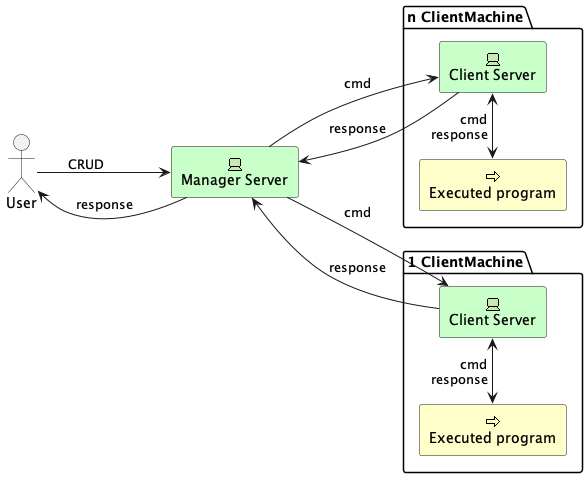
\includegraphics[height=0.4\textheight]{./part/Proyecto_ejecutivo/memoria_descriptiva/descripcionDelProyecto/manager/uml/systemConcept}
    \caption{Diagrama UML de despliegue del sistema}\label{fig:Diagrama UML de despliegue del sistema}
\end{figure}

El diagrama de despliegue del sistema en la~\cref{fig:Diagrama UML de despliegue del sistema} muestra que los actores en este sistema diseñado serán:
\begin{itemize}
    \item El servidor que contenga el programa \gls{Manager} permitirá la interacción de los usuarios con el sistema.
    Definirá, almacenará las tareas, las ejecutará en los sistemas remotos definidos y persistirá el resultado de dichas ejecuciones.
    \item Los servidores que contengan una copia del programa cliente \gls{Client} atenderán las llamadas del manager con el comando y lo ejecutará devolviendo los resultados.
    \item Los mismos servidores clientes contendrán los programas a ejecutar, pudiendo ser tantos como se deseen.
    En nuestro caso implementaremos el programa de control PID par aun motor de corriente continua.
\end{itemize}

La descripción de cada uno de los programas está compuesta de los siguientes puntos:

\begin{itemize}
    \item Diagrama de los despliegue: interacción entre componentes del subsistema.
    \item Diagrama de objetos: diagrama de su diseño \textit{DDD}.
    \item Casos de uso: descripción y diagrama de actividad.
    \item Estructura de carpetas para la organización del código.
\end{itemize}

\paragraph{Descripción constructiva del programa Manager}
\begin{figure}[H]
    \centering
    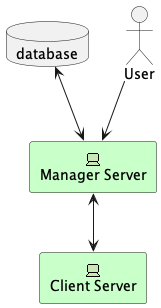
\includegraphics[height=0.4\textheight]{./part/Proyecto_ejecutivo/memoria_descriptiva/descripcionDelProyecto/manager/uml/managerServerConcept}
    \caption{Diagrama UML de despliegue del manager}\label{fig:Diagrama UML de despliegue del manager}
\end{figure}

\subparagraph{Dominio}

En el diagrama UML~\ref{fig:Diagrama UML de el dominio de manager} vemos que el dominio de Manager se compone de dos modulos: uno para las tareas y otro para los resultados. Vamos a ir explicando uno por uno:

\begin{figure}[H]
    \centering
    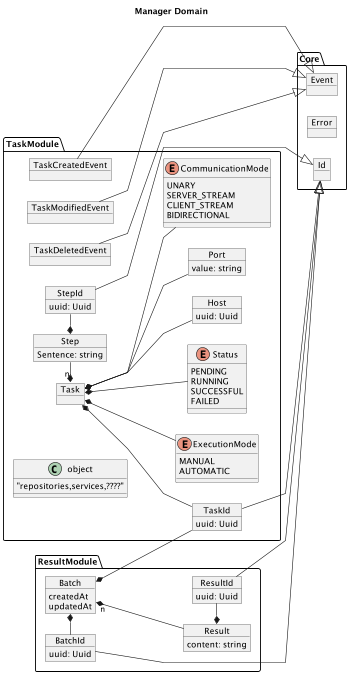
\includegraphics[height=0.4\textheight]{./part/Proyecto_ejecutivo/memoria_descriptiva/descripcionDelProyecto/manager/uml/managerDomain}
    \caption{Diagrama UML de el dominio de manager}\label{fig:Diagrama UML de el dominio de manager}
\end{figure}

\begin{itemize}
    \item CoreDomain
        \begin{itemize}
            \item \textbf{Id}: todos los ids extenderan de este id, contiene un uuid, no sabemos que paquete usaremos para generarlos, es una de las pocas dependencias externas que vamos a tener dentro del dominio y queremo encapsularla lo máximo posible por si hubera que cambiarla. Además de esta forma los ids de las entities no se confunden en su tipo. si por ejemplo buscas una task mediante un id que corresponde a un result, si fueran del mismo tipo daría lugar a confusión porque no lo encontraríamos pero no nos advertiría de nuestro error
            \item Event todos los eventos del sistema extenderan del evento este
        \end{itemize}
    \item TaskDomain
        \begin{itemize}
        \item \textbf{Task}: AggregateRoot
        \item \textbf{TaskId}
        \item \textbf{Host}: es un Value Object compuesto por el valor del host, es un string pero el Value Object garantiza que es un valor válido, si no devuelve un error
        \item \textbf{Port}: es un Value Object compuesto por el valor del puerto, es un string pero el Value Object garantiza que es un valor válido, si no devuelve un error
        \item \textbf{CommunicationMode}: es un enum para expresar esa tarea de las formas de comunicación posibles que hay entre dos servidores cual sera la utilizada
            \begin{itemize}
                \item UNARY
                \item SERVER\_STREAM
                \item CLIENT\_STREAM
                \item BIDIRECTIONAL
            \end{itemize}
        \item \textbf{ExecutionMode}: es un enum
        \begin{itemize}
            \item MANUAL
            \item AUTOMATIC
        \end{itemize}
        \item \textbf{Status}: es un enum \label{taskStatus}
        \begin{itemize}
            \item PENDING
            \item RUNNING
            \item SUCCESSFUL
            \item FAILED
        \end{itemize}
        \item \textbf{Step}: cada tarea puede componerse en distintos pasos. Por ejemplo queremos poder poner en marcha el motor durante 15 segudos y luego llevarlo a una posición de inicio
        \begin{itemize}
            \item \textbf{StepId}
            \item \textbf{sentence}: será un string de contenido libre que el servidor cliente ejecutará en su sistema, dependerá de él tener instalado dicho programa y corroborar que la sintaxis es la correcta
        \end{itemize}
        \item \textbf{TaskCreatedEvent}: Cuando se cree una tarea se emitirá un evento, habrá un manejador de eventos que actuará en consecuencia. Si es una tarea automatizada y el loop de ejecución está parado lo pondrá en marcha.
        \item \textbf{TaskModifiedEvent}: si una tarea es modificada se emitirá un evento, habrá un manejador de eventos que actuará en consecuencia. Si la tarea vuelve a ser puesta a pending, es automatizada y el loop de ejecución está parado lo pondrá en marcha
        \item \textbf{TaskDeletedEvent}: si una tarea es modificada se emitirá un evento, habrá un manejador de eventos que actuará en consecuencia.
    \end{itemize}
    \item \textbf{ResultDomain}
        \begin{itemize}
            \item \textbf{BatchId}
            \item \textbf{Batch}: aggregate root para referencial el conjunto de resultados correspondiente a la ejecución de una tarea. Una tarea se puede ejecutar varias veces, cada vez con distintos resultados. Para agruparlos necesitaremos este aggregate root
            \item \textbf{ResultId}
            \item \textbf{Result}: contendrá un string con el resultado en plano. Cada tarea y proceso tendrá a su disposición este strings para crear su propio formato de respuesta. Será tarea de cada cliente interpretarlos.
        \end{itemize}
\end{itemize}

\subparagraph{casos de uso}

Vamos a describir los casos de uso que podrán ejecutarse en el programa manager. Tenemos 2 Entities y dos aggregate root.

\begin{itemize}
    \item Task
    \subitem Step
    \item Batch
    \subitem Result
\end{itemize}

Vamos a hacer el \textit{CRUD} completo de Task, dentro de éste, se contempla la edición de los steps a través de Task ya que es su \textit{Aggregate Root} y por definición no se debe poder acceder a sus componentes si no es a través del \textit{Aggregate Root}. De Batch y Result no vamos a permitir el update por lógica de dominio este caso de uso no debe existir, ya que sus variables son autogeneradas en el momento de creación.

\textbf{Create Task}

La lógica de crear tareas se basará en la comprobación de que la información de entrada es correcta y suficiente, es decir, no hay parámetros opcionales. Por lo tanto deberán estar todos y ser validos. Esto se hará en la instanciación de los \textit{Value Object}. Si alguno de los datos no es válido el flujo se detendrá, devolviendo el error corespondiente al usario para que pueda subsanarlo y enviar una nueva petición.

\begin{figure}[H]
    \centering
    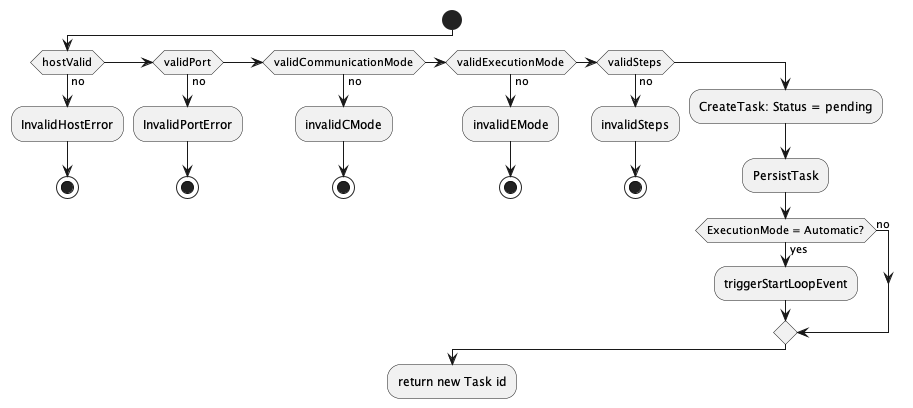
\includegraphics[height=0.2\textheight]{./part/Proyecto_ejecutivo/memoria_descriptiva/descripcionDelProyecto/manager/uml/createTaskUseCase}
    \caption{Use Case: Create Task}\label{fig:Use Case-Create Task}
\end{figure}

\textbf{Read Task}

La obtención de una Task se hará a través de su identificador \textit{UUID}. Se comprobará que efectivamente existe una Task con dicho identificador y de se devolverá el resultado de dicha búsqueda.

\begin{figure}[H]
    \centering
    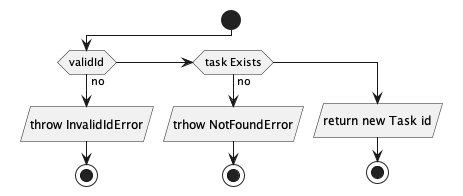
\includegraphics[height=0.15\textheight]{./part/Proyecto_ejecutivo/memoria_descriptiva/descripcionDelProyecto/manager/uml/getTaskUseCase}
    \caption{Use Case: Read Task}\label{fig:Use Case-Read Task}
\end{figure}

\textbf{Read Tasks}

Uno de los puntos más amplios en una \textit{API CRUD} es el filtrado de datos. No entra dentro del ámbito de este proyecto crear un sistema de filtrado que incluya la paginación. En este caso habría que crear una nomenclatura de filtros de cara al usuario y un sistema que los procese, devolviendo error ante un filtro erroneo o el listado de tareas que responda a dicho filtro. En nuestro caso devolveremos todas las tareas.

\textbf{Update Task}

A diferencia del flujo de creación en este caso si ha parámetros opcionales. Ya que este flujo equivale a lo que en REST se entiende como \textit{PATCH}, es decir una actualización parcial, los parámetros que no se reciban en la petición quedarán intactos. En un PUT el parámetro que no se recive se entiende que ha de ser eliminado.

\begin{figure}[H]
    \centering
    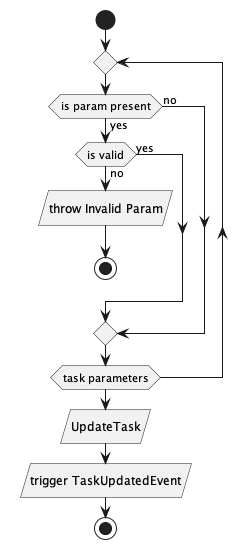
\includegraphics[height=0.4\textheight]{./part/Proyecto_ejecutivo/memoria_descriptiva/descripcionDelProyecto/manager/uml/updateTaskUseCase}
    \caption{Use Case: Update Task}\label{fig:Use Case-Update Task}
\end{figure}

\textbf{Delete Task}

En el flujo de eliminación de tareas, además de confirmar que la tarea que se desea eliminar existe, se añadirán más validaciones para garantizar al consistencia del sistema. No se permitirán eliminar tareas que estén en status \textit{RUNNING}\ref{taskStatus}

\begin{figure}[H]
    \centering
    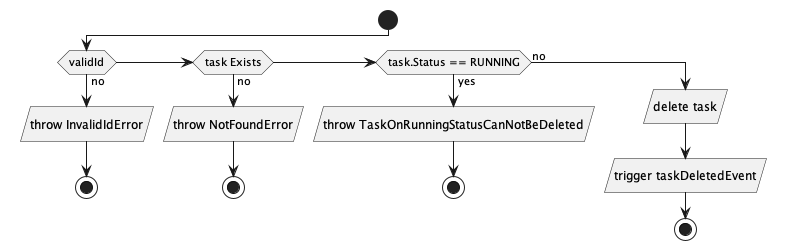
\includegraphics[height=0.2\textheight]{./part/Proyecto_ejecutivo/memoria_descriptiva/descripcionDelProyecto/manager/uml/deleteTaskUseCase}
    \caption{Use Case: Delete Task}\label{fig:Use Case-Delete Task}
\end{figure}

\textbf{TaskEventHandler}

Tanto en TaskCreatedEvent como TaskUpdatedEvent el handler va a ser el mismo. TaskDeletedEvent no será utilizado en este diseño inicial, pero se dejará preparado.


Con respecto al gestor de eventos vemos que tanto para la creación como para la actualización la lógica que estará presente será la comprobación de que si la tarea es de tipo automática, o se ha modificado a tipo automática; y si se acaba de crear, y por lo tanto el status es PENDING, o se ha modificado a dicho tipo; Entonces se comprobará que el loop de gestión de tareas está habilitado; de no ser así se habilitará.

\begin{figure}[H]
    \centering
    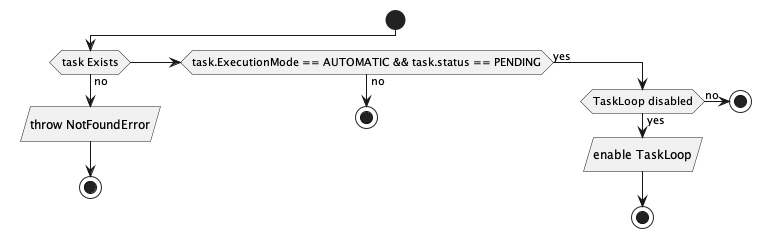
\includegraphics[height=0.2\textheight]{./part/Proyecto_ejecutivo/memoria_descriptiva/descripcionDelProyecto/manager/uml/taskEventHandlerUseCase}
    \caption{Use Case: TaskEventHandler}\label{fig:Use Case-TaskEventHandler}
\end{figure}

\textbf{TaskLoop: ejecutar tareas automáticas}

Una vez que el TaskEventHandler ponga en marcha el TaskLoop este obtendrá de base de datos todas las tareas automáticas pendientes y iterando sobre ellas lanzará un hilo de ejecución para ejecutarlas. Una vez terminadas todas volverá a intentar obtener tareas pendientes ya que en el periodo que haya estado ejecutandolas pueden haberse introducido nuevas. Si no hay más tareas pendientes el loop se desactivará.

Si hay que reseñar que este caso de uso es el core de la aplicación, donde se pondrá en juego la asincronía y todo el potencial del lenguaje. Es por tanto una primera versión del diseño. Igual que los otros casos de uso son lógica rutinaria que no debiera diferir mucho del diseño original, en este caso sí que podemos encontrarnos con lógicas que no estén previstas y por lo tanto haya que modificar. Todo quedará reflejado en la memoria explicativa de cambios \ref{subsec:memoria explicativa de cambios}

\begin{figure}[H]
    \centering
    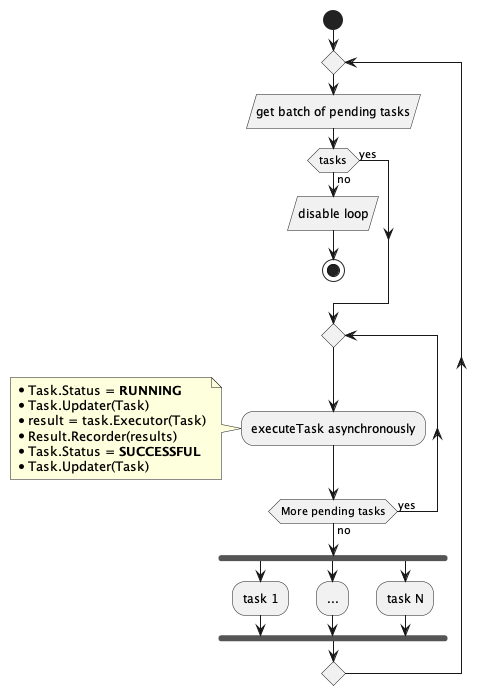
\includegraphics[height=0.3\textheight]{./part/Proyecto_ejecutivo/memoria_descriptiva/descripcionDelProyecto/manager/uml/executeTaskLoop}
    \caption{Use Case: TaskLoop}\label{fig:Use Case-TaskLoop}
\end{figure}

Atendiendo por tanto a esta posibilidad de cambio se hará uso de la arquitectura para desacoplarnos de dicha incertidumbre \textbf{TaskProcessor} que aparece en la figura \ref{fig:Use Case-TaskLoop} en color verde es el proceso asíncrono donde se hará uso del las gorutines que permiten la gestión de tareas asíncronas de forma sencilla. Lo definiremos como un puerto de salida e implementaremos un adaptador para encapsular esa incertidumbre.

Es de preveer que dentro de ese adaptador se implemente lógica que habrá de ser de negocio. Sin embargo, a no poder vislumbrarla con claridad, preferimos dejar pendiente de una refactorización. La refactorización posterior podrá ir introduciendo en dominio y limpiando dicho adaptador de el posible mal código resultado de la investigación mientras se construye, en vez de ensuciar el dominio y acoplar nuestro código base a esta incertidumbre.

A pesar de dicho desconocimiento inicial que nos impide diseñar con exactitud el flujo, El objetivo de este proyecto ejecutivo es hacer siempre una primera iteración en la medida que se pueda. Por lo tanto una primera iteración se puede ver en la figura \ref{fig:Use Case-Task Processor}

\begin{figure}[H]
    \centering
    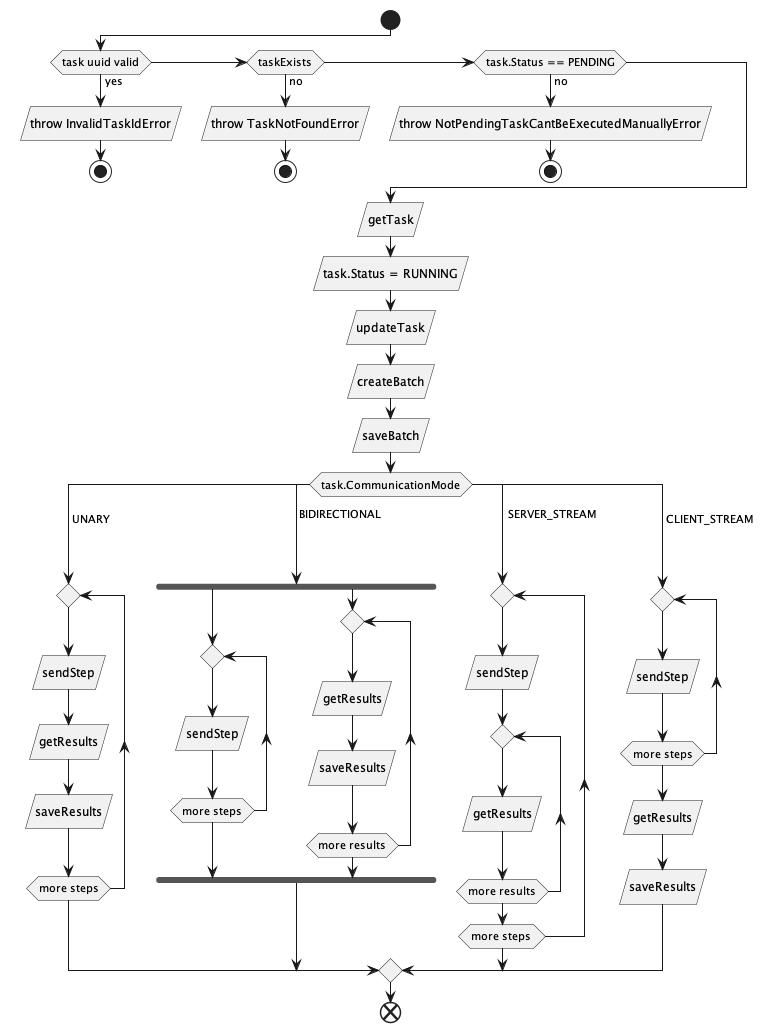
\includegraphics[height=0.55\textheight]{./part/Proyecto_ejecutivo/memoria_descriptiva/descripcionDelProyecto/manager/uml/1-TaskProcessor}
    \caption{Use Case: Task Processor}\label{fig:Use Case-Task Processor}
\end{figure}

Podemos ver que está muy acoplado a la interacción de los flujos de comunicación \textit{RPC}\ref{subsubsec:communications} de ahí nuestra incertidumbre al no haber trabajado todavía con dicha tecnología.

\textbf{Create Batch}

\begin{figure}[H]
    \centering
    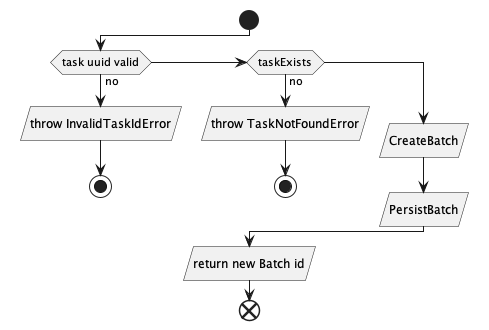
\includegraphics[height=0.2\textheight]{./part/Proyecto_ejecutivo/memoria_descriptiva/descripcionDelProyecto/manager/uml/createBatchUseCase}
    \caption{Use Case: Create Batch}\label{fig:Use Case: Create Batch}
\end{figure}

\textbf{Delete Batch}

\begin{figure}[H]
    \centering
    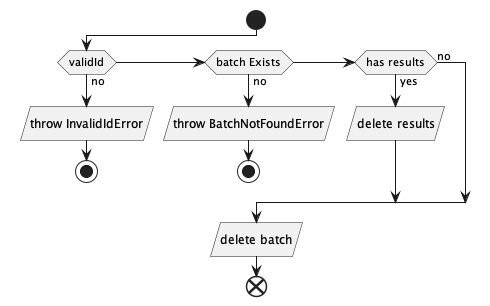
\includegraphics[height=0.2\textheight]{./part/Proyecto_ejecutivo/memoria_descriptiva/descripcionDelProyecto/manager/uml/deleteBatchUseCase}
    \caption{Use Case: Delete Batch}\label{fig:Use Case: Delete Batch}
\end{figure}

\textbf{Read batch}

\begin{figure}[H]
    \centering
    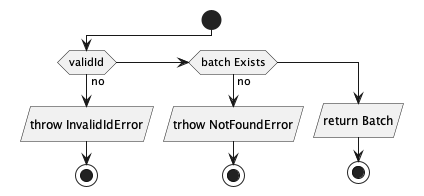
\includegraphics[height=0.2\textheight]{./part/Proyecto_ejecutivo/memoria_descriptiva/descripcionDelProyecto/manager/uml/getBatchUseCase}
    \caption{Use Case: Read Batch}\label{fig:Use Case: Read Batch}
\end{figure}

\textbf{Read batches of a Task}

Este caso de uso será necesario para obtener todos los Batches correspondientes a todas las ejecuciones de una misma tarea.

\begin{figure}[H]
    \centering
    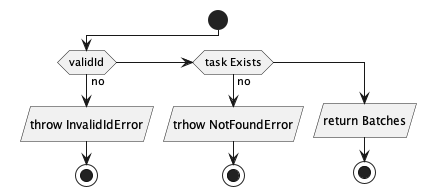
\includegraphics[height=0.2\textheight]{./part/Proyecto_ejecutivo/memoria_descriptiva/descripcionDelProyecto/manager/uml/getTaskBatchUseCase}
    \caption{Use Case: Read Batches of Task}\label{fig:Use Case-Read Batches of Task}
\end{figure}

\textbf{Obtener los results de un batch}

\begin{figure}[H]
    \centering
    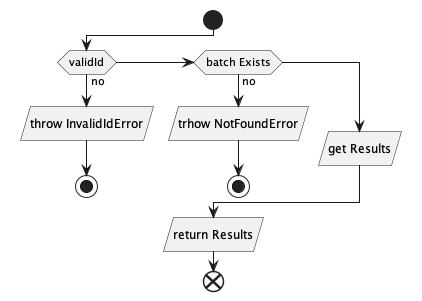
\includegraphics[height=0.2\textheight]{./part/Proyecto_ejecutivo/memoria_descriptiva/descripcionDelProyecto/manager/uml/getBatchResultsUseCase}
    \caption{Read Results of a Batch Use Case}\label{fig:Read Results of a Batch Use Case}
\end{figure}

\textbf{Execute task manually}

solo se puede ejecutar una tarea manual por vez, en este primer diseño. El motivo es que como se quiere graficar en tiempo real la respuesta, por ejemplo para monitorizar la velocidad del motor en tiempo real, no queremos meternos en la complejidad de graficar varios resultados a la vez.

\begin{figure}[H]
    \centering
    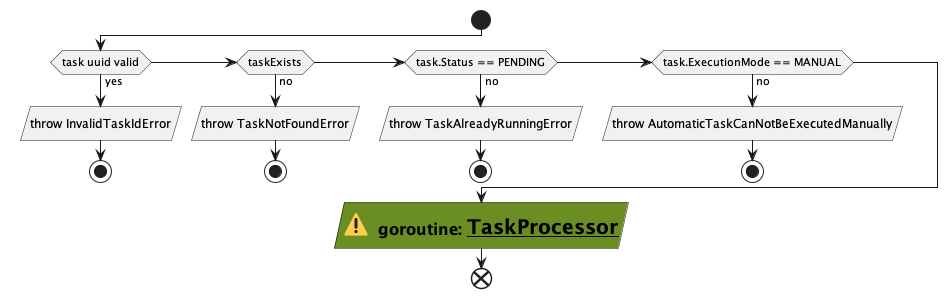
\includegraphics[height=0.2\textheight]{./part/Proyecto_ejecutivo/memoria_descriptiva/descripcionDelProyecto/manager/uml/1-executeTaskManual}
    \caption{Use Case: Execute Task Manually}\label{fig:Use Case-Execute Task Manually}
\end{figure}

El diagrama de secuencia para el caso de que una tarea sea de tipo BIDIRECTIONAL se puede apreciar en el diagrama \ref{fig:executeTaskManualInteraction}. Este es el caso que utilizaremos por ejemplo para el control en velocidad y posición del motor de corriente continua. Se enviará una consigna y se recibirán resultados hasta que el cliente envíe la orden de detener dicho control. Para otros tipos más simples, por ejemplo, ejecutar manualmente la tarea de configurar el PID, simplemente será de tipo UNARY, se enviará una request y se obtendrá una respuesta.

\begin{figure}[H]
    \centering
    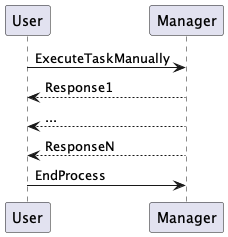
\includegraphics[height=0.2\textheight]{./part/Proyecto_ejecutivo/memoria_descriptiva/descripcionDelProyecto/manager/uml/1-ExecuteTaskManuallyInteraction}
    \caption{Execute task manually interaction}\label{fig:executeTaskManualInteraction}
\end{figure}

\subparagraph{estructura de carpetas}

Una de las partes mas importantes de un proyecto de software es que la estructura de carpetas hable sobre cómo está diseñado el software, sobre de qué va el software. qué es lo que hace y sobre que componentes interactua

En el proyecto constará de 4 carpetas principales
\dirtree{%
    .1 Project .
        .2 Adapter.
        .2 Application.
        .2 Domain.
        .2 Bootstrap.
}

Bootstrap será donde hagamos la composición de la aplicación, es decir la inyección de dependencias.

Vamos a desplegar la estructura capa por capa

\textbf{Adapters}

\dirtree{%
.1 Adapter.
    .2 in.
        .3 GRPC.
            .4 CreateEntityGrpcCall.
        .3 Console.
            .4 CreateEntityTerminalCommand.
    .2 out.
        .3 Email.
            .4 SendEmailOnCreationImplementation (*1).
        .3 Mysql.
            .4 SaveEntityImplementation (*2).
}

\textbf{Aplicación}

\dirtree{%
.1 Application.
    .2 Port.
        .3 in.
            .4 Entity.
                .5 CreateUseCase.
                    .6 CreateCommand.
                        .7 CreateCommand (using sendEmail param in this example).
                        .7 CreateUseCase.
                    .6 SomeEventHandler.
                        .7 CreationEvent.
                        .7 CreationEventUseCase.
        .3 out.
            .4 Email.
                .5 SendEmailConCreation (interface for *1).
}

\textbf{Dominio}

\dirtree{%
.1 Domain.
    .2 Core.
        .3 Id.
        .3 Event.
        .3 Error.
    .2 Task.
        .3 Id.
        .3 Task.
        .3 Host.
        .3 Port.
        .3 CommunicationMode.
        .3 ExecutionMode.
        .3 Status.
        .3 Step.
            .4 Id.
            .4 StepEntity.
            .4 StepVo.
            .4 Repository.
                .5 Find.
                .5 Save.
                .5 Search.
                .5 Delete.
                .5 Update.
            .4 Service.
                .5 Finder.
                .5 Creator.
                .5 Updater.
                .5 Eraser.
                .5 Searcher.
        .3 Repository.
            .4 Find.
            .4 Save.
            .4 Search.
            .4 Delete.
            .4 Update.
        .3 Service.
            .4 Finder.
            .4 Creator.
            .4 Updater.
            .4 Eraser.
            .4 Searcher.
    .2 Result.
}



\paragraph{Descripción constructiva del programa Cliente}
\begin{figure}[H]
    \centering
    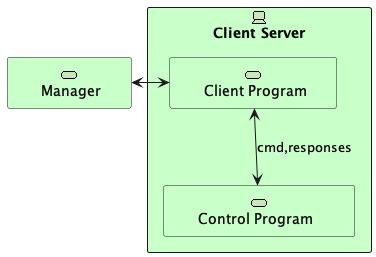
\includegraphics[height=0.3\textheight]{./part/Proyecto_ejecutivo/memoria_descriptiva/descripcionDelProyecto/client/uml/clientServerConcept}
    \caption[Diagrama componentes]{}\label{fig:clientServerConcept}
\end{figure}

\subparagraph{Dominio}

Hay que tener en cuenta que en este programa será casi todo infrestructura. ya que una vez recepcionado el comando mediante el RPC
solo habrá que ejecutarlo en el servidor cliente y será tarea del cliente configurar dicho servidor para que dicho comando exista. Será tarea del programa a ejecutar interpretar dicho comando y trasnformar ese comando y esos argumentos en un dominio interno. Por ejemplo un programa típico de consola en un sistema UNIX

\begin{verbatim}
    ./runMyComand --arg=arg1 --argN=argN
\end{verbatim}


Las posibilidades son tantas como comandos haya instalados en el servidor cliente. En nuestro caso podremos mandar a ejecutar todos los comandos que queramos que vengan previamente instalados en un sistema UNIX y además el programa de control donde podremos interactuar con el motor de corriente continua

\begin{verbatim}
    ./pidControl --velocity=30rpm
    ./pidControl --position=180deg
    ./pidControl --setP=1
    ./pidControl --setI=0
    ./pidControl --setD=0
    ./pidControl --enabled=true
    ./pidControl --enabled=false
\end{verbatim}

aquí podemos ver por ejemplo los comándos básicos de un control pid que podremos ejecutar. En la descripción del programa de control y su dominio lo veremos en más detalle


\begin{figure}[H]
    \centering
    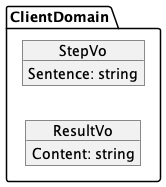
\includegraphics[height=0.4\textheight]{./part/Proyecto_ejecutivo/memoria_descriptiva/descripcionDelProyecto/client/uml/clientDomain}
    \caption[Diagrama de objetos de dominio]{}\label{fig:clientDomain}
\end{figure}

\begin{itemize}
    \item StepDomain
    \begin{itemize}
        \item StepVo
    \end{itemize}
    \item ResultDomain
    \begin{itemize}
        \item ResultVo
    \end{itemize}
\end{itemize}

\subparagraph{casos de uso}

Vamos a describir los casos de uso que podrán ejecutarse en el programa client. En este caso no tendremos Entities porque no necesitamos identificadores.
Tendremos los Value Objects para los steps que nos llegaran a modo de request y el necesario para responder. En este sistema no hay persistencia.

\begin{itemize}
    \item StepVo
    \item ResultVo
\end{itemize}

\textbf{execute Unary Step}

Centrando en un caso de uso de este tipo de steps en nuestro programa de control sirve por ejemplo para establecer un parámetro de control del PID. Cualquiera de los siguientes.
\begin{verbatim}
    ./pidControl --velocity=30rpm
\end{verbatim}

Podemos ver en~\ref{fig:executeUnaryStep} el diagrama de flujo que responde a este caso de uso

\begin{figure}[H]
    \centering
    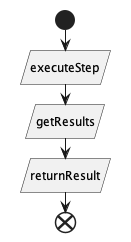
\includegraphics[height=0.2\textheight]{./part/Proyecto_ejecutivo/memoria_descriptiva/descripcionDelProyecto/client/uml/executeUnaryStep}
    \caption[Diagrama de objetos de dominio]{}\label{fig:executeUnaryStep}
\end{figure}

\textbf{execute ClientStream Step}

Centrando en un caso de uso de este tipo de steps en nuestro programa de control sirve por ejemplo para establecer una configuración completa con una sola llamada para nuestro PID:
\begin{verbatim}
    ./pidControl --velocity=30rpm
    ./pidControl --position=180deg
    ./pidControl --setP=1
    ./pidControl --setI=0
    ./pidControl --setD=0
\end{verbatim}

Podemos ver en~\ref{fig:executeClientStreamStep} el diagrama de flujo que responde a este caso de uso

\begin{figure}[H]
    \centering
    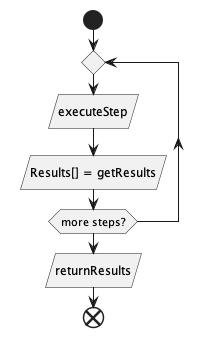
\includegraphics[height=0.2\textheight]{./part/Proyecto_ejecutivo/memoria_descriptiva/descripcionDelProyecto/client/uml/executeClientStreamStep}
    \caption[Diagrama de objetos de dominio]{}\label{fig:executeClientStreamStep}
\end{figure}

\textbf{execute ServerStream Step}

Centrando en un caso de uso de este tipo de steps en nuestro programa de control sirve por ejemplo para habilitar el control del pid durante un determinado tiempo e ir devolviendo el estado la variable de control
\begin{verbatim}
    ./pidControl --enabled=true --time=10s
\end{verbatim}

O dejar el control activado indefinidamente hasta que llege otra request de tipo Unary que lo detenga

\begin{verbatim}
    ./pidControl --enabled=false
\end{verbatim}

Podemos ver en~\ref{fig:executeServerStreamStep} el diagrama de flujo que responde a este caso de uso

\begin{figure}[H]
    \centering
    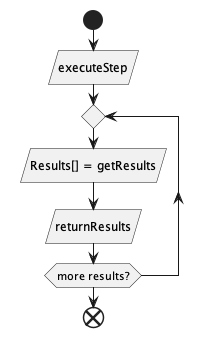
\includegraphics[height=0.2\textheight]{./part/Proyecto_ejecutivo/memoria_descriptiva/descripcionDelProyecto/client/uml/executeServerStreamStep}
    \caption[Diagrama de objetos de dominio]{}\label{fig:executeServerStreamStep}
\end{figure}

\textbf{execute Bidirectional Step}

Usando el ejemplo anterior, si no queremos habilitar el control indefinidamente y deshabilitarlo mediante otra request podemos usar este caso de uso.

\begin{verbatim}
    ./pidControl --enabled=true --time=10s
\end{verbatim}

y posteriormente cuando el Cliente decida.

\begin{verbatim}
    ./pidControl --enabled=false
\end{verbatim}

Este caso de uso es el que utilizaremos para el control manual.

Podemos ver en~\ref{fig:executeBidiStep} el diagrama de flujo que responde a este caso de uso

\begin{figure}[H]
    \centering
    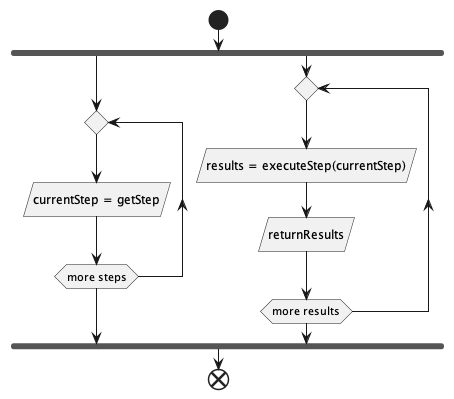
\includegraphics[height=0.2\textheight]{./part/Proyecto_ejecutivo/memoria_descriptiva/descripcionDelProyecto/client/uml/executeBidiStep}
    \caption[Diagrama de objetos de dominio]{}\label{fig:executeBidiStep}
\end{figure}

\subparagraph{estructura de carpetas}

En el proyecto constará de 4 carpetas principales

\tiny
\dirtree{%
    .1 Project .
        .2 Domain.
        .2 Application.
        .2 Adapter.
        .2 Bootstrap.
}
\normalsize

\textbf{Dominio}

\begin{figure}[H]
    \tiny
\dirtree{%
    .1 Domain.
        .2 Step.
            .3 StepVo.
            .3 Repository.
                .4 consoleWrite.
            .3 Services.
                .4 Executor.
        .2 Result.
            .3 ResultVo.
}
\normalsize
    \caption[Diagrama de objetos de dominio]{}\label{fig:1-ClientDomainFolderStructure}
\end{figure}

\textbf{Aplicación}

\tiny
\dirtree{%
.1 Application.
    .2 Port.
        .3 in.
            .4 Step.
                .5 Execute.
                    .6 Command.
                    .6 UseCase.
}
\normalsize

\textbf{Adapters}

\tiny
\dirtree{%
    .1 Adapter.
        .2 in.
            .3 GRPC.
                .4 Harán uso de los useCases de aplicación cuando llegue una request RPC.
            .3 Console.
                .4 Por ejemplo si quisieramos ejecutar los casos de uso mediante terminal.
        .2 out.
            .3 console.
                .4 implementación de los repository de llamada a los servidores clientes.
}
\normalsize







\paragraph{Descripción constructiva del programa de Control}
Casos de uso todas las funciones del engine y diseñarlo para que la infra sea a través de consola de comandos (preparando para que luego debido a la comunicación rpc devolver los datos sea muy complicado si lo dividimos en otro comando y decidimos absorver este dominio)

El sistema está pensado para que el programa a ejecutar sea de libre decisión del cliente. pero vamos a aprovechar la oportunidad para crear un programa de control y profundizar tanto en el uso del lenguaje como en los conocimientos relacionados con este master. En concreto el control automático. Uno do los programas que podrá ejecutar será un control PID.



\begin{figure}[H]
    \centering
    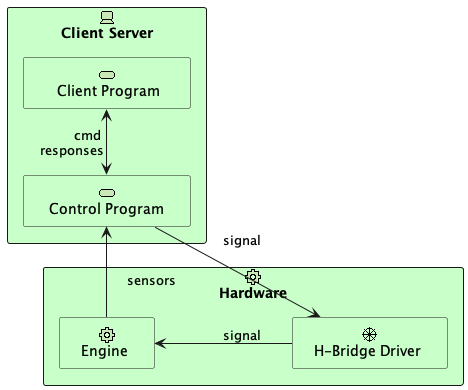
\includegraphics[height=0.2\textheight]{./part/Proyecto_ejecutivo/memoria_descriptiva/descripcionDelProyecto/control/uml/controlConcept}
    \caption{Control: Diagrama UML de despliegue}\label{fig:Control-Diagrama UML de despliegue}
\end{figure}

\subparagraph{Dominio}

\begin{figure}[H]
    \centering
    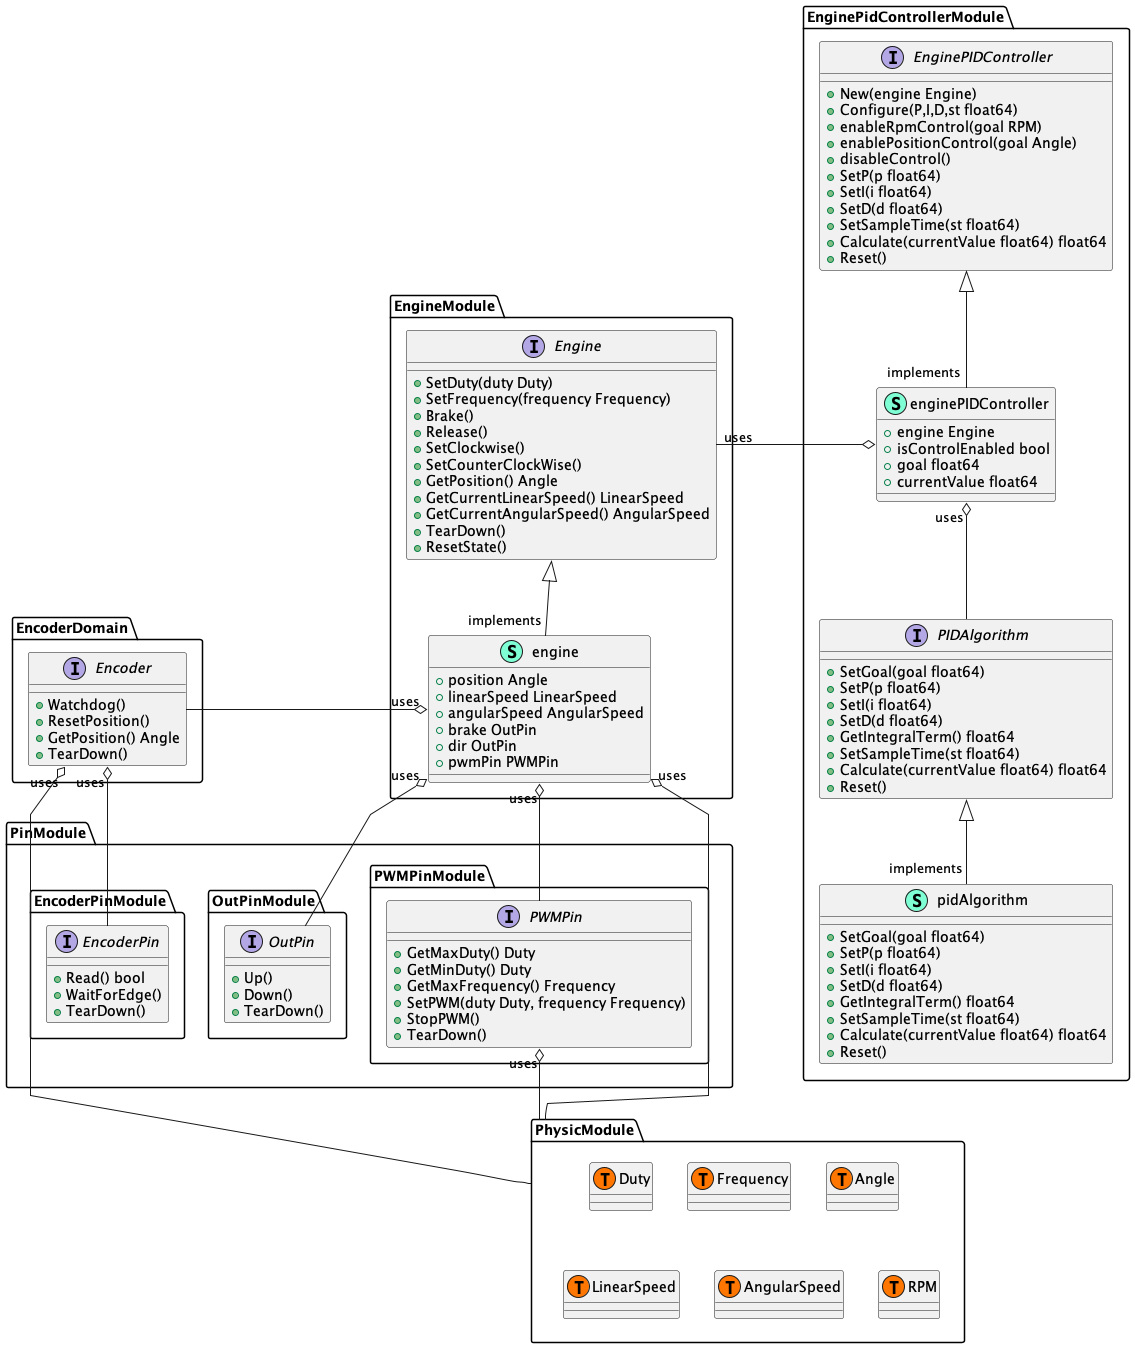
\includegraphics[height=0.45\textheight]{./part/Proyecto_ejecutivo/memoria_descriptiva/descripcionDelProyecto/control/uml/controlDomain}
    \caption{Control: Diagrama UML de el dominio}\label{fig:Control-Diagrama UML de el dominio}
\end{figure}

\begin{itemize}
    \item PhysicModule: contendrá todas las variables físicas, son interfaces de int y floats que usaremos para garantizar la congruencia en las operaciones. Aunque los tipos sean float hay variables que no pueden operar entre sí sin atender a su realidad física, es decir sus unidades.
    \item PinModule: para abstraernos del sistema donde se ejecute el código crearemos la abstracción de el hardware necesario para atender a interfaz física de un motor:
    \begin{itemize}
        \item EncoderPinModule: sabemos que vamos a necesitar un pin de entrada tipo pull de entrada y esperar a los flancos de subida que entrarán del encoder. Ya sea en los hardwares comerciales más conocidos como arduino o raspberry como cualquier otro.
        \item OutPinModule: para activar o desactivar frenos y triggers de dirección necesitaremos pin de salida
        \item PWMPinModule: para tener un control PWM necesitaremos un pin que nos permita salida pero con una frecuencia y un ciclo de trabajo.
    \end{itemize}
    \item EncoderModule: estará compuesto por dos pines de tipo Encoder para leer los pulsos y calcular si está en una dirección
    \item EngineModule: este modulo contendrá tanto la interfaz del motor como la implementación, donde haciendo uso de los pines calculará y contendrá las variables intrínsecas del motor.
    \item EnginePIDControllerModule: contendrá todo lo relativo al controlador PId. El controlador usará una instancia de Engine y una instancia de PIDAlgorithm
\end{itemize}

\subparagraph{Casos de uso}

Los casos de usos actuarán sobre El objeto de dominio EnginePIDController, que en este caso al no haber base de datos ni identificadores serán ValueObjects. Particularmente en nuestro programa solo instanciaremos uno. No implementaremos un patrón singleton sobre ellos debido a que podría desearse controlar varios motores a la vez si el hardware lo permitiera.

\textbf{Configure PID}

El primer paso a ejecutar antes de habilitar el control PID será sintonizarlo.

\begin{figure}[H]
    \centering
    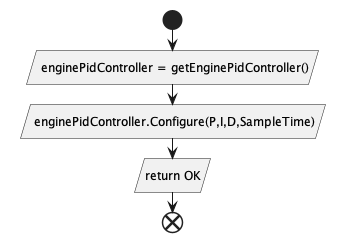
\includegraphics[height=0.2\textheight]{./part/Proyecto_ejecutivo/memoria_descriptiva/descripcionDelProyecto/control/uml/configurePID}
    \caption{Use Case: Configure PID}\label{fig:Use Case-Configure PID}
\end{figure}

\textbf{Enable RPM control}

Cuando se habilita el control rpm se genera una goRutine, es decir una nuevo proceso que se quedará ejecutando hasta que se ejecute el caso de uso Disable Control

\begin{figure}[H]
    \centering
    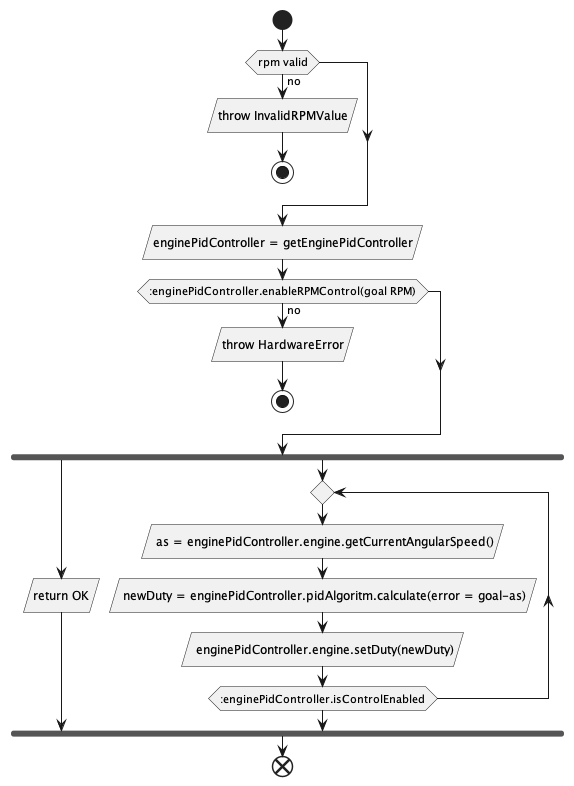
\includegraphics[height=0.5\textheight]{./part/Proyecto_ejecutivo/memoria_descriptiva/descripcionDelProyecto/control/uml/enableRPMControl}
    \caption{Use Case: Enable RPM control}\label{fig:Use Case- Enable RPM control}
\end{figure}

\textbf{Enable Position control}

\begin{figure}[H]
    \centering
    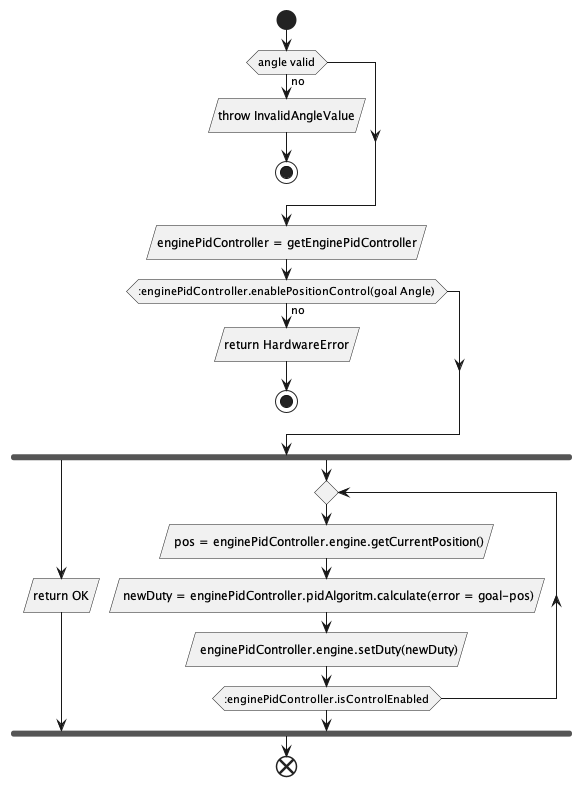
\includegraphics[height=0.4\textheight]{./part/Proyecto_ejecutivo/memoria_descriptiva/descripcionDelProyecto/control/uml/enablePositionControl}
    \caption{Use Case: Enable Position control}\label{fig:Use Case- Enable Position control}
\end{figure}

\textbf{Disable control}

\begin{figure}[H]
    \centering
    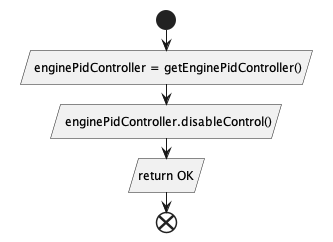
\includegraphics[height=0.2\textheight]{./part/Proyecto_ejecutivo/memoria_descriptiva/descripcionDelProyecto/control/uml/disableControl}
    \caption{Use Case: Disable control}\label{fig:Use Case- Disable control}
\end{figure}

\subparagraph{estructura de carpetas}

\begin{figure}[H]
    \setlength{\DTbaselineskip}{10pt}
    \DTsetlength{0.2em}{1em}{0.2em}{0.4pt}{1.6pt}
    \dirtree{%
        .1 Project .
            .2 Domain.
            .2 Application.
            .2 Adapter.
            .2 Bootstrap.
    }
    \caption{Control: Estructura de carpetas de proyecto}\label{fig:Control- Estructura de carpetas de proyecto}
\end{figure}

\textbf{Dominio}

\begin{figure}[H]
    \setlength{\DTbaselineskip}{10pt}
    \DTsetlength{0.2em}{1em}{0.2em}{0.4pt}{1.6pt}
    \dirtree{%
        .1 Domain.
            .2 EnginePidController.
                .3 \textcolor{blue}{EnginePidController.go}.
                .3 Service.
                    .4 \textcolor{blue}{Configurator.go}.
                    .4 \textcolor{blue}{RPMControllerActivator.go}.
                    .4 \textcolor{blue}{PositionControllerActivator.go}.
                    .4 \textcolor{blue}{ControlDisabler.go}.
            .2 Engine.
                .3 \textcolor{blue}{EngineVo.go}.
                .3 Repository.
                    .3 \textcolor{blue}{Find.go}.
            .2 Encoder.
                .3 \textcolor{blue}{Encoder.go}.
            .2 Pin.
                .3 EncoderPin.
                    .4 \textcolor{blue}{EncoderPinInterface.go}.
                .3 OutPin.
                    .4 \textcolor{blue}{OutPinInterface.go}.
                .3 PWMPin.
                    .4 \textcolor{blue}{PWMPinInterface.go}.
            .2 Physic.
                .3 \textcolor{blue}{Angle.go}.
                .3 \textcolor{blue}{LinearSpeed.go}.
                .3 \textcolor{blue}{AngularSpeed.go}.
                .3 \textcolor{blue}{Frequency.go}.
                .3 \textcolor{blue}{Duty.go}.
    }
    \caption{Control: Estructura de carpetas de Dominio}\label{fig:Control- Estructura de carpetas de Dominio}
\end{figure}

\textbf{Aplicación}

\begin{figure}[H]
    \setlength{\DTbaselineskip}{10pt}
    \DTsetlength{0.2em}{1em}{0.2em}{0.4pt}{1.6pt}
    \dirtree{%
        .1 Application.
            .2 Port.
            .3 in.
                .4 EnginePidController.
                    .5 ConfigureCommand.
                        .6 \textcolor{blue}{Command.go}.
                        .6 \textcolor{blue}{UseCase.go}.
                    .5 EnableRpmControlCommand.
                        .6 \textcolor{blue}{Command.go}.
                        .6 \textcolor{blue}{UseCase.go}.
                    .5 EnablePositionControlCommand.
                        .6 \textcolor{blue}{Command.go}.
                        .6 \textcolor{blue}{UseCase.go}.
                    .5 DisableCommand.
                        .6 \textcolor{blue}{Command.go}.
                        .6 \textcolor{blue}{UseCase.go}.
    }
    \caption{Control: Estructura de carpetas de Aplicación}\label{fig:Control-Estructura de carpetas de Aplicación}
\end{figure}

\textbf{Adapters}

\begin{figure}[H]
    \setlength{\DTbaselineskip}{10pt}
    \DTsetlength{0.2em}{1em}{0.2em}{0.4pt}{1.6pt}
    \dirtree{%
        .1 Adapter.
            .2 in.
                .3 GRPC.
                    .4 Harán uso de los useCases de aplicación cuando llegue una request RPC.
                .3 Console.
                    .4 Por ejemplo si quisieramos ejecutar los casos de uso mediante terminal.
            .2 out.
                .3 pin.
                    .4 implementación con librerías para actuar sobre los pines, Se buscará una librería que pueda ser configurada para actuar sobre pines de varias plataformas.
    }
    \caption{Control: Estructura de carpetas de Infraestructura}\label{fig:Control-Estructura de carpetas de Infraestructura}
\end{figure}






